%%% In this section, you will describe all of the various artifacts that you will generate and maintain during the project life cycle. Describe the purpose of each item below, how the content will be generated, where it will be stored, how often it will be updated, etc. Replace the default text for each section with your own description. Reword this paragraph as appropriate.

\subsection{Major Documentation Deliverables}

\subsubsection{Project Charter}
The project charter will be updated at the end of each sprint if necessary. The circumstance in which this document will be updated is based off the sprint review, and we as a team will check if there is a change in any aspect of our project, and will update accordingly. The initial version will be delivered October 11th, 2021. The final version will be delivered at the beginning of May 2022.

\subsubsection{System Requirements Specification}
This document will be updated after the discussion with team members and sponsor about the product requirements, and/or when there is any change in current requirements or addtion of new features. The initial version will be delivered at the end of October 2021, and the final version will be delivered in May 2022.

\subsubsection{Architectural Design Specification}
The document's initial version will be delivered November 15, 2021. The final version will be delivered in May 2022.

\subsubsection{Detailed Design Specification}
This document will be maintained and updated as we continue to develop the web application. If we make any change in the software functionality then we will update this accordingly. The document's initial version will be delivered at the end of February 2022. The final version will be delivered in May 2022. 

\subsection{Recurring Sprint Items}
The following items will be documented and maintained during each individual sprint.

\subsubsection{Product Backlog}
All requirements and update that are collected during the discussion between team members and Professor Chris Conly/sponsor will be added to the product backlog from the SRS. The items will be prioritized based on its urgency of getting feedback and the relation to other items. However, in case the sponsor prioritizes any feature, the hierarchy may be change accordingly. Any decision on the project will be decided based on group vote and the sponsor's advice. We will use GitHub to maintain and share the product backlog with team members and stakeholders.

\subsubsection{Sprint Planning}
Each sprint will be planned following the end of the previous sprint during a meeting with all team members. There will be eight sprints.

\subsubsection{Sprint Goal}
The sprint goal will be decided by the team as a whole. The team can meet with the customer for feedback, or the sprint plan will be emailed to them for feedback.

\subsubsection{Sprint Backlog}
The team leader and their assistent will choose which product backlog items make their way into the sprint backlog. GitHub Projects will be used to maintain the backlog items.

\subsubsection{Task Breakdown}
Each team member will voluntarily claim their tasks, and they will also document the time spent on each task in their Engineering Notebook.

% \subsubsection{Sprint Burn Down Charts}
% Who will be responsible for generating the burn down charts for each sprint? How will they be able to access the total amount of effort expended by each individual team member? What format will the burn down chart use (include an example burn down chart below).

% %%%%%%%%%%%%%%%%%%%%%%%%%%%%%%%%%%%%%%%%%%%%%%%%%%%%%%%%%%
% %  BE SURE TO UPDATE THE IMAGE CAPTION
% \begin{figure}[h!]
%     \centering
%     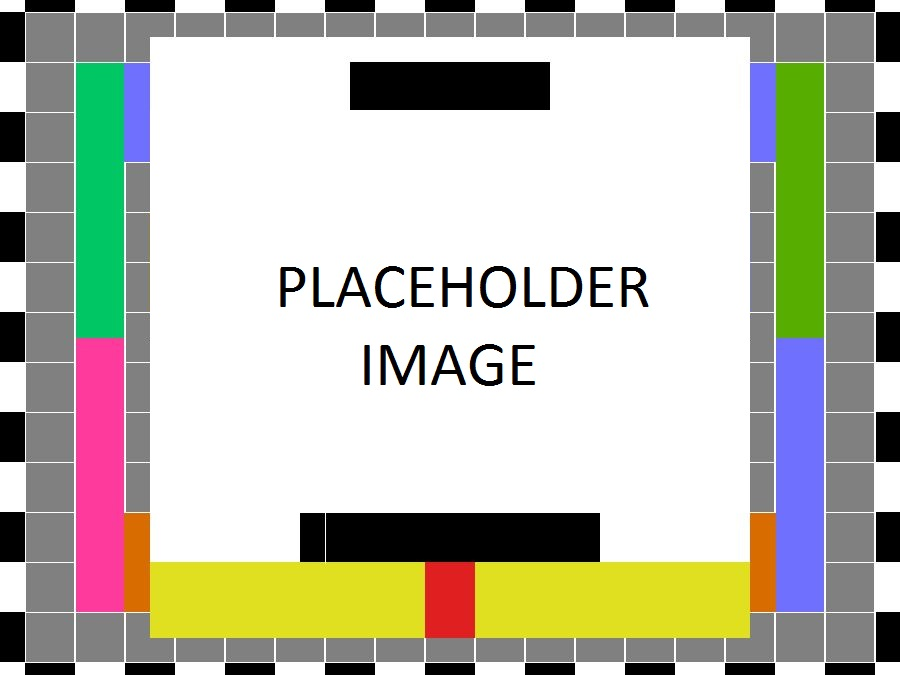
\includegraphics[width=0.5\textwidth]{images/test_image} % Image
%     \caption{Example sprint burn down chart} % Caption
% \end{figure}

\subsubsection{Sprint Retrospective}
The team will meet and document everything that was done between the team members. The disussion will happen before the next sprint starts. Every feature will be sorted by which group members worked on it, and if multiple members worked on an item or was worked on during a group meeting. This will be due before the start of each sprint.

\subsubsection{Individual Status Reports}
We will create the individual Status Report based off the sample report provided by the professor. It will be reported at the end of each sprint. The report will contain the spring goal, sprint backlog, individual time expenditures, individual retrospective, a peer review, and if needed a burndown chart. 

\subsubsection{Engineering Notebooks}
The Engineering Notebook will be updated by each member at the end of the day that they worked on the project. The minimum amount of pages will vary per sprint. Each interval is a week long. The team will keep each member accountable by reminding everyone to update their ENB at the end of every week. Any teammate that is available can sign off as a "witness" for each ENB page.

\subsection{Closeout Materials}
The following materials, in addition to major documentation deliverables, will be provided to the customer upon project closeout.

\subsubsection{System Prototype}
There will be a working web application where users will be able to make their own degree plan. The PAT and FAT will be decided later on as we start developing the project.

\subsubsection{Project Poster}
The project poster will be devlivered at the mid-March 2022. The final dimensions will be decided when the poster is being created. The poster as of now will include pictures of the web application, and will be designed in a manner where the viewers will be able to get a better understanding of the features provided by our application.

\subsubsection{Web Page}
Our project is the web-based application that is accessible to public, therfore, the homepage will basically be the project home page. The final product will be delivered at the end of semester in May 2022.

\subsubsection{Demo Video}
The demo video will be a sreen recording of the web application in use. The demo will create a sample user and show how to use the application and create a degree plan. 

\subsubsection{Source Code}
The source code will be maintained using Git and GitHub. Source code will be provided to the customer as a ZIP file. The project will also be open source with the license GPL-3.0. The lisense terms are listed in a file called "LICENSE" in the source code ZIP file.

\subsubsection{Source Code Documentation}
Documentation will be required for all classes, methods, functions, and variables. A documentation generator will be used, a specific tool will be decided on at a later time. The format of the final documentation will decided later.

\subsubsection{Hardware Schematics}
The project is fully web-based application, so we do not require any hardware schematics.

\subsubsection{CAD files}
The project is fully web-based application, so we do not require CAD files.

\subsubsection{Installation Scripts}
There will be a readme file with instructions and screenshots. Perhaps even some copy and
    paste lines for installation.

\subsubsection{User Manual}
A digital user manual and a demo video explaining all instructions will be available for the customer.
